\ylDisplay{Liiklejad} % Ülesande nimi
{Tundmatu autor} % Autor
{lõppvoor} % Voor
{2015} % Aasta
{P 10} % Ülesande nr.
{3} % Raskustase
{
% Teema: Mehaanika

\ifStatement
 Sirgel teel sörgib Ants kiirusega $v_A = 7,0$ km/h. Samal teel sõidab Birgit mopeediga samas suunas kiirusega $v_B = 25$ km/h. Teist sellega lõikuvat sirget teed mööda sõidab jalgrattaga Gerd kiirusega $v_G = 20$ km/h. Vahemaa Antsu ja Gerdi vahel jääb kogu aeg võrdseks vahemaaga Gerdi ja Birgiti vahel. Leidke Gerdi kiirus Birgiti suhtes.
\fi

\ifHint
Antsu, Birgiti ja Gerdi asukhad moodustavad igal ajahetkel võrdhaarse kolmnurga, mille alus asub Antsu ja Birgiti poolt kasutataval teel. Gerdi liikumine koosneb kahest komponendist: Antsu ja Birgitiga paralleelses sihis liikumisest ja nende liikumissuunaga risti liikumisest.
\fi

\ifSolution
\begin{center}
	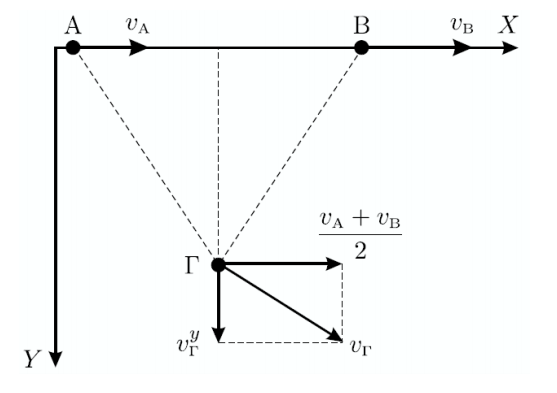
\includegraphics[width=0.5\linewidth]{2015-v3p-10-lah.PNG}
\end{center}
Antsu, Birgiti ja Gerdi asukhad moodustavad igal ajahetkel võrdhaarse kolmnurga, mille alus lebab Antsu ja Birgiti poolt kasutataval teel (vt. joonist). 
Olgu X-telg paralleelne selle teega ning Y-telg sellega risti. Siis järgmised võrrandid kirjeldavad liiklejate koordinaatide muutusi:
\begin{center}
Antsu jaoks: $x_A(t) = x_A ^0 + v_At$, $y_A(t) = 0$;
\end{center}
\begin{center}
Birgiti jaoks: $x_B(t) = x_B ^0 + v_Bt$, $y_B(t) = 0$;
\end{center}
\begin{center}
Gerdi jaoks: $x_G(t) = \frac{x_A ^0 + x_B ^0}{2} + \frac{v_A + v_B}{2}t$, $y_G(t) = y_G ^0(t) + v_G ^y t$.
\end{center}
Siin ülemindeksiga "0" tähistame esialgseid koordinaate ning tähtedega $A, B, G$ tähistame suurusi vastavalt Antsu, Birgiti ja Gerdi jaoks. $v_G ^y$ on Gerdi kiiruse projektsioon Y teljele. Seos $x_G(t)$ jaoks on tuletatud asjaolulst, et Gerd on alati võrdhaarse kolmnurga tipus, mis on vastamisi kolmnurga alusega. Siit järeldub, et Gerdi kiiruse projektsioon X-teljele on $\frac{v_A + v_B }{2}$.
Me teame Gerdi kiiruse suurust, millesse pannustavad selle komponendid:
\begin{center}
$v_g ^2 = (\frac{v_A + v_B})^2 + (v_G ^y)^2$ 
\end{center}
Seetõttu Gerdi kiiruse projektsioon Y-teljele on
\begin{center}
$v_G^y =\sqrt{v_G^y - (\frac{v_A + v_B}{2})^2}$.
\end{center}
Nüüd teame Gerdi kiiruse mõlemaid projektsioone ning saame leida tema kiiruse Birgiti suhtes. Kasutades Pythagorase teoreemi kiiruste kolmnurga jaoks leiame, et
\begin{center}
$v_{suht} ^2 = (v_A - \frac{v_a + v_b}{2})^2 + (v_G ^y)^2$.
\end{center}
Asendades $v_G ^y$ saame
\begin{center}
$v_{suht} = \sqrt{v_G ^2 - v_A \cdot v_B } = 15$ km/h
\end{center}
\fi
}